\section{Task Definition}
To collect vehicle data of the Fleet Management System (FMS) and provide IP-based access, a dedicated device has to be developed. It acts as a gateway (communication bridge) and connects the internal CAN-Bus to the on-board network router via LAN or WLAN.


A general block diagram of the system is shown in \cref{fig:constellation_HW}.

\medskip
\begin{figure}[h!]
	\centering
	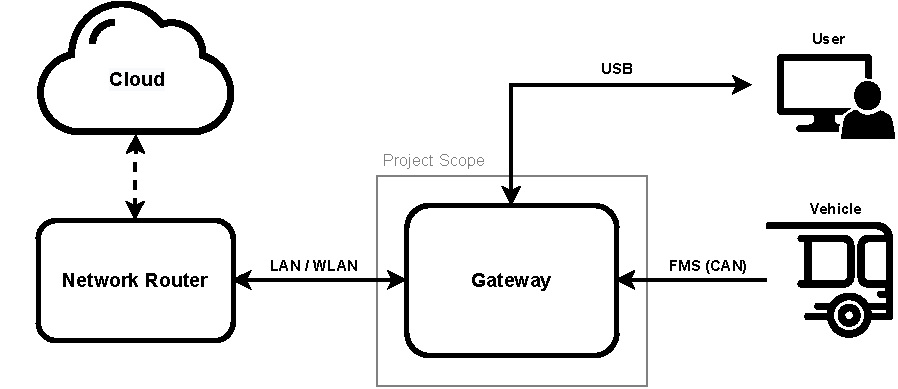
\includegraphics[height=5cm]{images/Block_Diagram}
	\caption{System Block Diagram}
	%\vspace{-2ex}
	%\caption*{\textbf{Source:} Original task definition}
	\label{fig:constellation_HW}
\end{figure}

FMS-Packets are received and processed by the gateway. A configurable filter decides which packets get forwarded and limits the maximal transmission update rate. The network router acts as a receiver, which can upload the information  over the internet to a cloud-based system.
Device settings as well as the filter configuration

To gather additional motion data of the vehicle, an inertial measurement unit (IMU) should be integrated.

\begin{itemize}
	\item bla 1
	\item bla 2
	\item bla 3
\end{itemize}

Various use cases were defined in \cref{sec:use_cases}.